\section{Opis struktury projektu}
\subsection{Architektura systemu}
System został zbudowany w oparciu o wzorzec MVC (Model-Widok-Kontroler):
\begin{itemize}
\item \textbf{Model}: Baza danych SQLite + klasy dziedziny (Produkt, Transakcja itp.)
\item \textbf{Widok}: Interfejs użytkownika zrealizowany w Swing
\item \textbf{Kontroler}: Logika biznesowa aplikacji
\end{itemize}


\subsection{Diagram klas}
\begin{figure}[H]
\centering
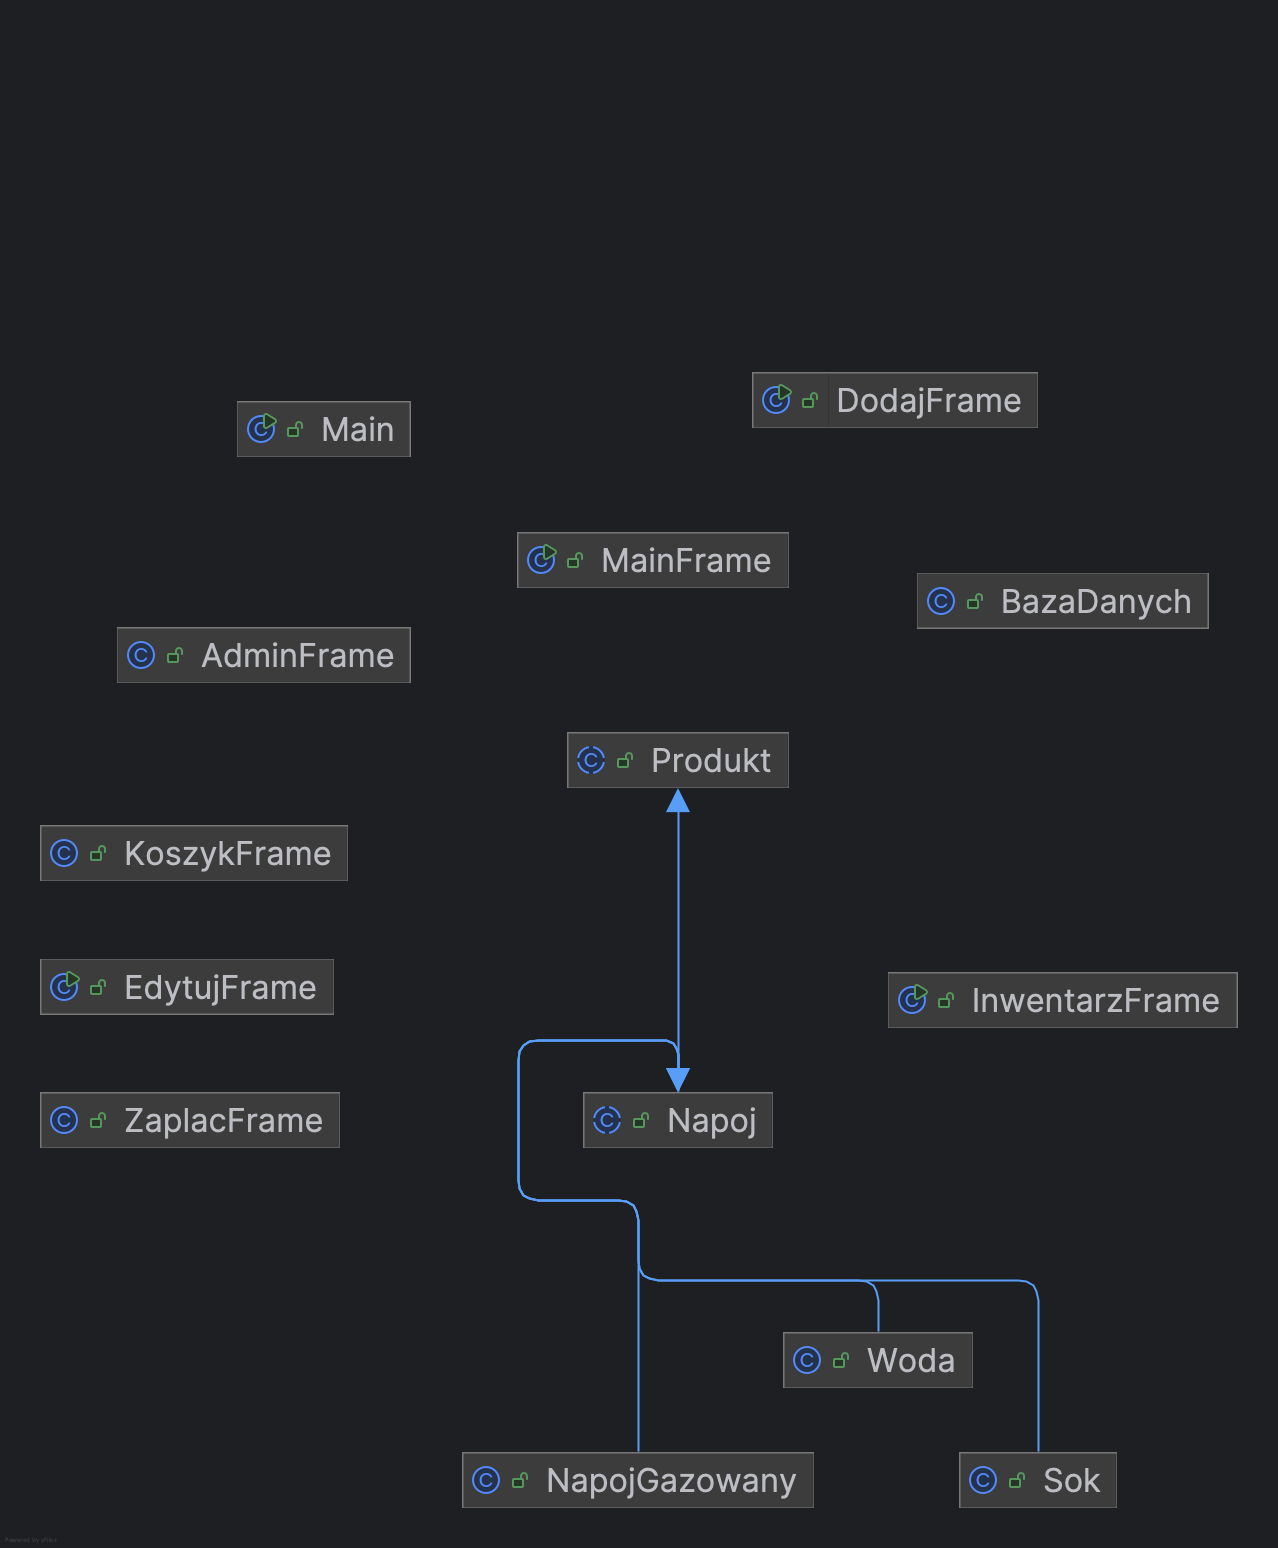
\includegraphics[width=0.9\textwidth]{figures/class_diagram.png}
\caption{Diagram głównych klas systemu}
\label{fig:class_diagram}
\end{figure}

\subsection{Hierarchia dziedziczenia}
System wykorzystuje mechanizm dziedziczenia do modelowania różnych typów produktów. Główna hierarchia klas przedstawia się następująco:

\begin{figure}[H]
\centering
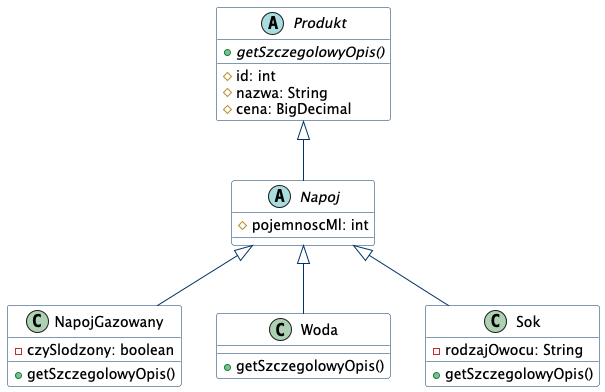
\includegraphics[width=0.7\textwidth]{figures/inheritance_diagram.png}
\caption{Hierarchia dziedziczenia klas produktów}
\label{fig:inheritance_diagram}
\end{figure}

\subsubsection{Klasa bazowa Produkt}
Klasa abstrakcyjna \texttt{Produkt} stanowi podstawę hierarchii:

\begin{lstlisting}[style=javaStyle]
public abstract class Produkt {
    protected int id;
    protected String nazwa;
    protected BigDecimal cena;
    
    public abstract String getSzczegolowyOpis();
}
\end{lstlisting}

\subsubsection{Klasa Napoj}
Klasa \texttt{Napoj} dziedziczy po \texttt{Produkt}, rozszerzając ją o specyficzne dla napojów właściwości:

\begin{lstlisting}[style=javaStyle]
public abstract class Napoj extends Produkt {
    protected int pojemnoscMl;
    
    public Napoj(int id, String nazwa, BigDecimal cena, int pojemnoscMl) {
        super(id, nazwa, cena);
        this.pojemnoscMl = pojemnoscMl;
    }
}
\end{lstlisting}

\subsubsection{Klasy konkretne}
Specyficzne typy napojów dziedziczą po klasie \texttt{Napoj}, implementując własne wersje metody \texttt{getSzczegolowyOpis()}:

\begin{itemize}
\item \texttt{NapojGazowany} - dodaje informację o słodzeniu
\begin{lstlisting}[style=javaStyle, firstnumber=1]
public class NapojGazowany extends Napoj {
    private boolean czySlodzony;
    
    @Override
    public String getSzczegolowyOpis() {
        return String.format("Napój gazowany: %s\nPojemność: %d ml\n(%s)",
            nazwa, pojemnoscMl, czySlodzony ? "słodzony" : "bez cukru");
    }
}
\end{lstlisting}

\item \texttt{Sok} - dodaje informację o rodzaju owocu
\item \texttt{Woda} - podstawowa implementacja dla wody
\end{itemize}

\subsubsection{Zalety zastosowanego podejścia}
\begin{itemize}
\item \textbf{Reużywalność kodu}: Wspólne właściwości są zdefiniowane w klasach nadrzędnych
\item \textbf{Polimorfizm}: Możliwość traktowania różnych typów produktów jednolicie
\item \textbf{Rozszerzalność}: Łatwe dodawanie nowych typów produktów
\end{itemize}

Przykład wykorzystania polimorfizmu w klasie \texttt{BazaDanych}:

\begin{lstlisting}[style=javaStyle]
public static List<Produkt> pobierzWszystkieProdukty() {
    List<Produkt> produkty = new ArrayList<>();
    // ...
    switch (typProduktu) {
        case "GAZOWANY":
            produkty.add(new NapojGazowany(...));
            break;
        case "SOK":
            produkty.add(new Sok(...));
            break;
        // ...
    }
    return produkty;
}
\end{lstlisting}


Kluczowe klasy systemu:
\begin{itemize}
\item \textbf{MainFrame}: Główne okno aplikacji
\item \textbf{Produkt}: Klasa abstrakcyjna reprezentująca produkt
\item \textbf{Napoj}, \textbf{NapojGazowany}, \textbf{Woda}, \textbf{Sok}: Hierarchia klas produktów
\item \textbf{KoszykFrame}: Obsługa koszyka zakupowego
\item \textbf{ZaplacFrame}: Logika płatności
\item \textbf{BazaDanych}: Warstwa dostępu do danych
\end{itemize}



\subsection{Baza danych}
System wykorzystuje lekką bazę danych SQLite z następującymi tabelami:
\begin{itemize}
\item \textbf{produkty} (id, nazwa, cena, typ, ilość)
\item \textbf{detale\_napoje} (id\_produktu, pojemność\_ml)
\item \textbf{transakcje} (id, data, produkty, kwota, metoda\_płatności)
\end{itemize}

\begin{figure}[H]
\centering
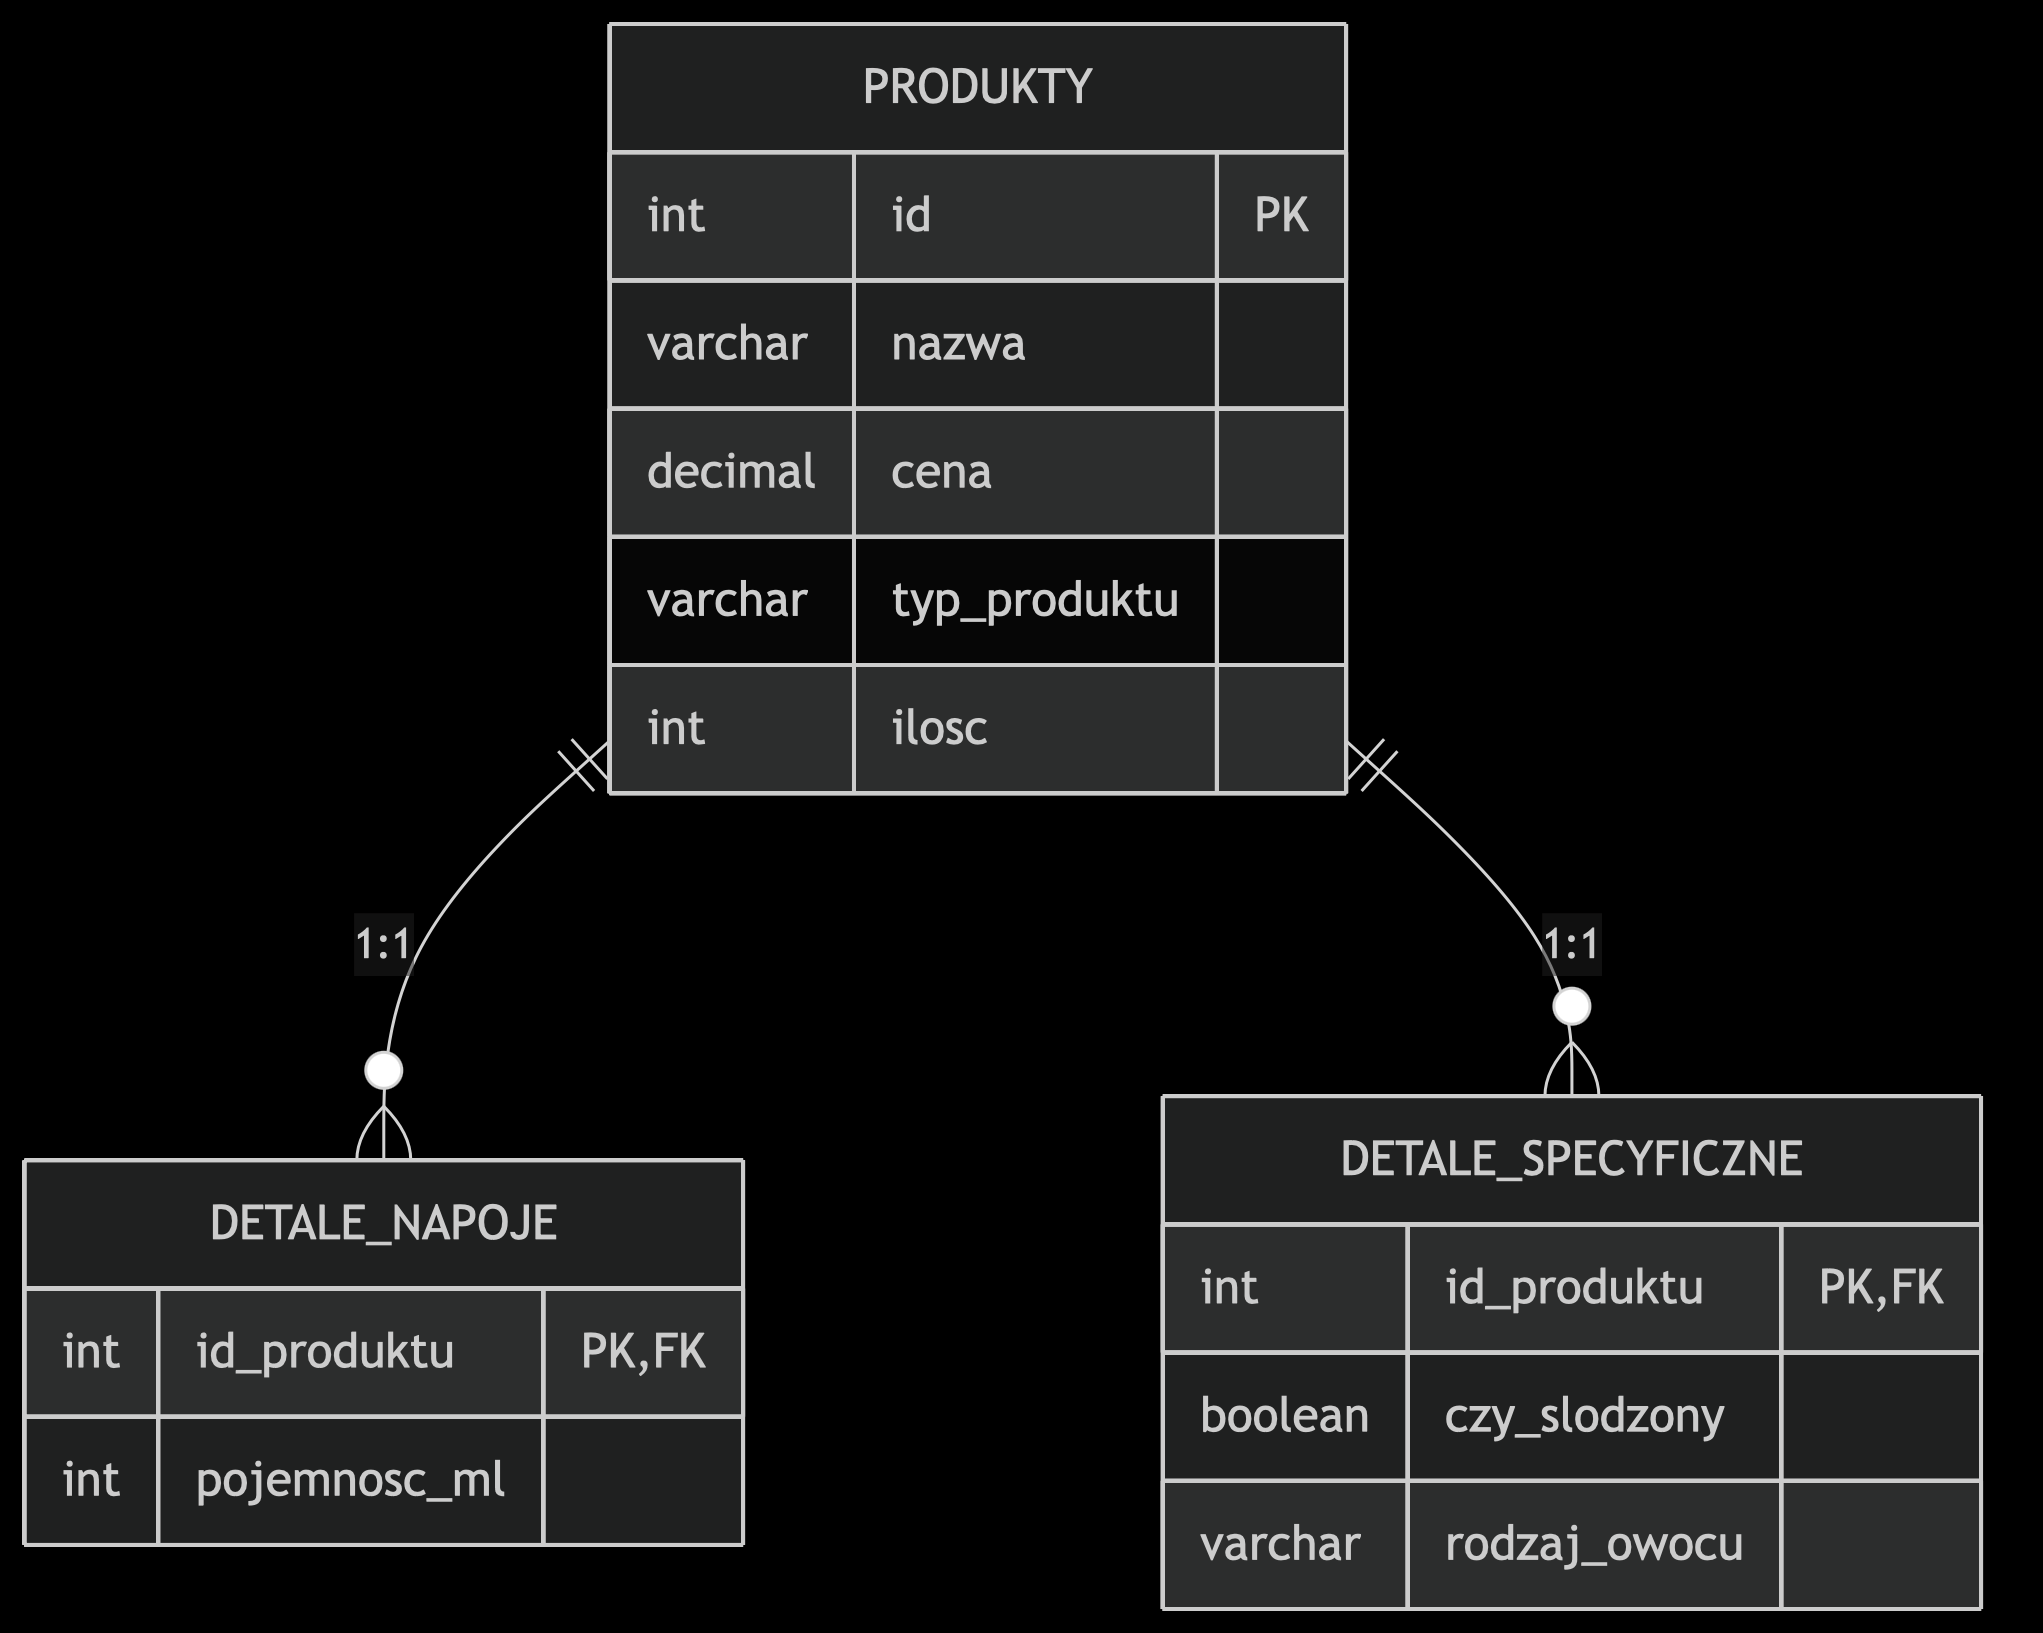
\includegraphics[width=0.8\textwidth]{figures/erd_diagram.png}
\caption{Diagram ERD bazy danych}
\label{fig:erd_diagram}
\end{figure}